\begin{figure*}[hbtp]
  \centering
  \subfigure[Overall result]{
    \label{fig:8020-runtime--mean}
    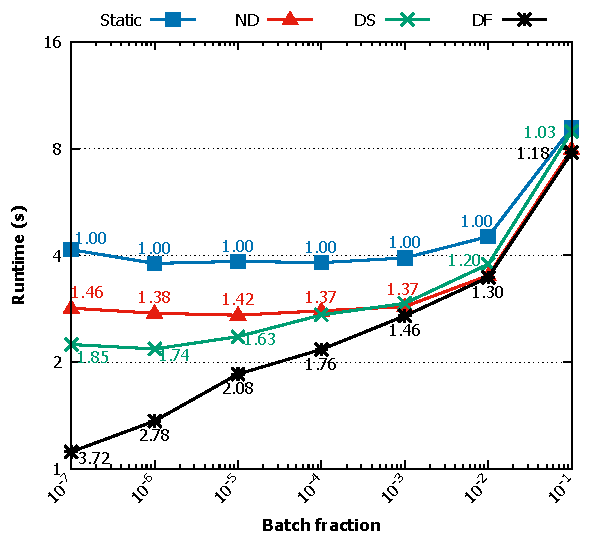
\includegraphics[width=0.38\linewidth]{out/8020-runtime-mean.pdf}
  }
  \subfigure[Results on each graph]{
    \label{fig:8020-runtime--all}
    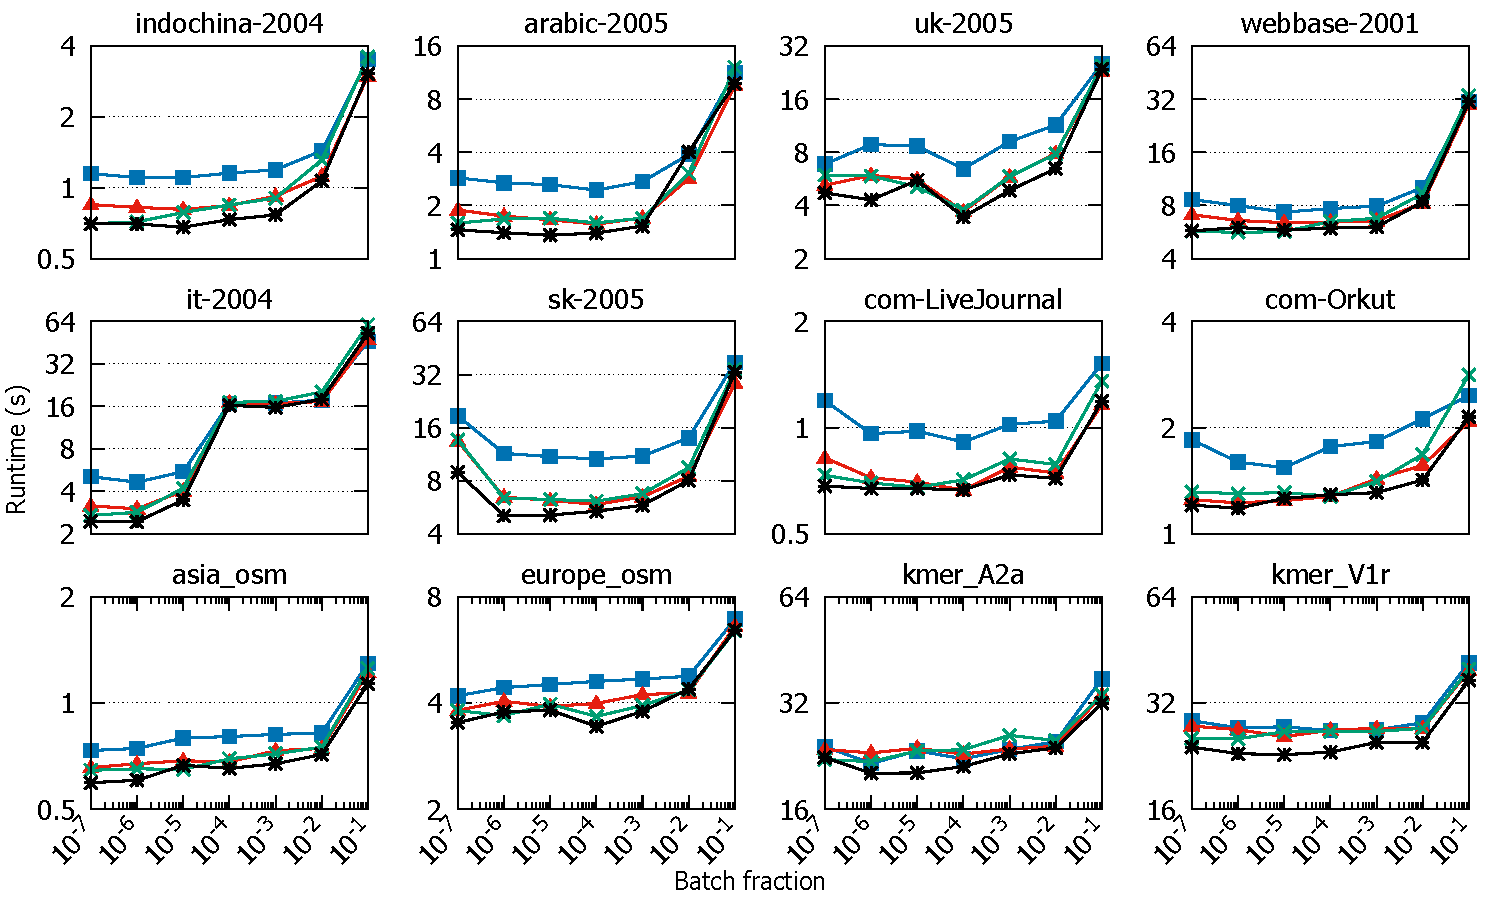
\includegraphics[width=0.58\linewidth]{out/8020-runtime-all.pdf}
  } \\[-2ex]
  \caption{Runtime (logarithmic scale) of our multicore implementation of \textit{Naive-dynamic (ND)}, \textit{Delta-screening (DS)}, and \textit{Dynamic Frontier (DF) Leiden}, compared to \textit{Static Leiden} \cite{sahu2024fast}, on large\ignore{(static)} graphs with randomly generated batch updates. The size of these batch updates ranges from $10^{-7}|E|$ to $0.1|E|$ in multiples of $10$, with the updates comprising $80\%$ edge insertions and $20\%$ edge deletions to simulate realistic dynamic graph changes. The right subfigure shows the runtime of each algorithm for individual graphs in the dataset, while the left subfigure displays overall runtimes using the geometric mean for consistent scaling across graphs.\ignore{Furthermore,} The speedup of each algorithm compared to Static Leiden is indicated on the respective lines.}
  \label{fig:8020-runtime}
\end{figure*}
